\documentclass[utf8]{frontiersSCNS} % for Science, Engineering and Humanities and Social Sciences articles
\usepackage{url,hyperref,lineno,microtype,subcaption}
\usepackage[onehalfspacing]{setspace}
\usepackage{graphicx}

\linenumbers


\def\keyFont{\fontsize{8}{11}\helveticabold }
\def\firstAuthorLast{Mannella {et~al.}} %use et al only if is more than 1 author

\def\Authors{Francesco Mannella$^{1}$*, Vieri Santucci$^{1}$, Eszter Somogyi$^{2}$, Lisa Jacquey$^{2}$,
Kevin J. O'Regan$^{2}$, Gianluca Baldassarre$^{1}$  }
% Affiliations should be keyed to the author's name with superscript numbers and be listed as follows: Laboratory, Institute, Department, Organization, City, State abbreviation (USA, Canada, Australia), and Country (without detailed address information such as city zip codes or street names).
% If one of the authors has a change of address, list the new address below the correspondence details using a superscript symbol and use the same symbol to indicate the author in the author list.
\def\Address{
$^{1}$Institute of cognitive sciences and technologies, \\National Research Council - CNR,  Rome, Italy \\
$^{2}$Laboratoire Psychologie de la Perception (UMR 8158), \\Paris Descartes - CPSC, Paris, France 
}
% The Corresponding Author should be marked with an asterisk
% Provide the exact contact address (this time including street name and city zip code) and email of the corresponding author
\def\corrAuthor{
Francesco Mannella\\
Institute of cognitive sciences and technologies\\
Via San Martino della Battaglia, 44\\
00185 Roma, Italia
}

\def\corrEmail{francesco.mannella@gmail.com}


\begin{document}
\onecolumn
\firstpage{1}

\title[Know your body through intrinsic goals]{Know your body through intrinsic goals} 


\author[\firstAuthorLast ]{\Authors} %This field will be automatically populated
\address{} %This field will be automatically populated
\correspondance{} %This field will be automatically populated
\extraAuth{}% If there are more than 1 corresponding author, comment this line and uncomment the next one.
%\extraAuth{corresponding Author2 \\ Laboratory X2, Institute X2, Department X2, Organization X2, Street X2, City X2 , State XX2 (only USA, Canada and Australia), Zip Code2, X2 Country X2, email2@uni2.edu}


\maketitle


\begin{abstract}
\section{}
The first `object' that newborn children start start to play with is their own body. This activity allows them to autonomously form a sensorimotor map and a repertoire of actions that constitutes the core of future cognitive and motor development. In this work we propose a computational model incorporating the hypothesis that this acquisition of early knowledge is not guided by random motor-babbling, but rather by goals autonomously generated and set on the basis of intrinsic motivations. During the initial motor-babbling, the system forms representations of sensory events. When the agent realises the possibility to re-activate those representations through its motor behaviour, it will be intrinsically motivated to improve its competence in obtaining those specific events. More precisely, the discovered events become intrinsic goals that guide both the learning and the selection of motor actions. The model is based on five components: (1) a competitive neural network, supporting the acquisition of abstract representations based on experienced changes in the
sensory input; (2) a selector that on the basis on competence-based intrinsic motivations (CB-IMs) determines the pursued goal and which motor resources will be trained to obtain that goal; (3) an echo-state neural network that controls the movements of the robot and supports the acquisition of the motor skills; (4) a predictor of the accomplishment of the pursued goal, used to measure the improvement of the system competence; (5) the generator of the CB-IM signal that biases the activity of the selector. The model is tested as the controller of a simulated simple planar robot composed of two kinematic 3DoF arms exploring own body in a 2D environment. Sensory information from self-touching is used by the system to form goals and guide skill learning. Results are presented, together with their possible implications for ongoing empirical experiments with human babies. Moreover, the model will be discussed in relation to possible applications to design new open-ended learning robotic architectures able to act in unstructured environments.
 

\tiny
 \keyFont{ \section{Keywords:} developmental robotics, developmental psychology, intrinsic motivations, goals, body schema} %All article types: you may provide up to 8 keywords; at least 5 are mandatory.
\end{abstract}

\section{Introduction}
\label{sec:Intro}
The first ``object'' that newborn children start to play with is their own body. This activity, that starts even in the fetus and continues for many years after birth \citep{Bremner2008}, determines the formation of a ``body schema'' (cit.), a sensorimotor map and a repertoire of actions that constitute the core of future cognitive and motor development. [TODO, Kevin]

If we observe children in their first months, they seem to alternate phases of rest to phases of random activity of the limbs that gradually became more controlled and targeted during their development. Differently from this empirical evidence, in this work we propose a computational model incorporating the hypothesis that early knowledge in children is not acquired through random motor-babbling, but guided by self-generated goals, autonomously set on the basis of intrinsic motivations (IMs).

The concept of IMs was introduced in animal psychology during the 1950s and then extended in human psychology \citep{Berlyne1950,White1959,Berlyne1960,deci1985,Ryan2000}  to describe a set of motivations that were incompatible with the Hullian theory of drives \citep{Hull1943} where motivations were strictly connected to the satiation of primary needs. Different experiments \citep[e.g.][]{Harlow1950,Montgomery1954,Kish1955,Glow1978} showed how exploration, novel or surprising neutral stimuli and even the possibility to affect the environment are able to modify the behaviour of the agents driving the acquisition of knowledge and skills in the absence of tasks directly established by biological fitness. Further neurophysiological research \citep[e.g.][]{Chiodo1980,Horvitz2000,Redgrave2006} showed how IMs can be linked to neuromodulators activity, and in particular to dopamine. These results highlighted the role of IMs in enhancing neural plasticity and driving the learning of new skills. Following biological inspiration, IMs has been also introduced in machine learning \citep[e.g.][]{Barto2004,Schmidhuber2010} and developmental robotics \citep[e.g.][]{Oudeyer2007a,BaldassarreMirolliBook} to foster the autonomous development of artificial agents and the open-ended learning of repertoires of skills. Depending on their functions and mechanisms, different typologies of IMs have been identified \citep{Oudeyer2007b,Santucci2013a,Barto2013} and broadly into two main groups \citep{Baldassarre2014}: (1) knowledge-based IMs (KB-IMs), divided in (1a) novelty based IMs related to novel non-experienced stimuli, and (1b) prediction-based IMs, related to the violation of the agent's predictions; and (2) competence-based IMs (CB-IMs) related to action, i.e. to the agent's competence to change the world and accomplish self-defined $goals$. In their first implementations in computational research, IMs have been used to generate the learning signal for autonomous skills acquisition \citep{Oudeyer2007a,Hart2011,Mirolli2013,Kompella2015}. Recent research has started to use IMs for the autonomous generation and/or selection of $goals$ which can then drive the acquisition of skills \citep{Merrick2012,Baranes2013,Santucci2016} and the optimisation of learning processes in high-dimensional action spaces with redundant robot controllers \citep{Baranes2013,Rolf2014}.

Together with IMs, $goals$ are a crucial element for the presented model. Here, in consonance with computational and empirical perspectives \citep{Russell2003,Thill2013}, goals are intended as agent's internal representations of a world/body state or event (or of a set of them), with these properties: (a) the agent can keep the representation active even in the absence of the corresponding state or event; (b) the representation has the power to focus the behaviour of the agent towards the accomplishment of the goal and to generate a learning signal when the world state matches the goal (``goal-matching'').

Our hypothesis is that goals and IMs play an important role even in the early phases of knowledge acquisition, i.e. in the first months after birth. In particular, the infant initial motor-babbling results in the formation of sensory events representations. When the baby discovers (through further random activity) the possibility to re-activate the same representations through its behaviour, this will generate a CB-IM signal for obtaining those specific sensory events. More precisely, the discovered events become intrinsic goals that guide both the learning and the selection of motor actions. 

Given the important role of IMs in enhancing exploration, a different hypothesis on the development of early knowledge could exclude the involvement of an high-level construct such as goals.\\
TODO] Kevin, you should develop here the hypothesis that we discussed with you in the past (what we initially called the `oudeyer hypothesis').\\
If we remember some key points of it were as follows.\\
The agent is endowed with a repertoire of actions.\\
The agent is able to recognise a certain number of `interesting' outcomes.\\
The problem of its development is to learn a repertoire of action-outcome contingencies on the basis of intrinsic motivations.\\
The acquisition process works as follows.\\
The agent explores the environment with its actions.\\
When an interesting outcome is detected, the agent memorise in its repertoire the action-outcome contingency just experienced.\\
The action and the perceptual experience involved in the contingecy now receive a high motivation for exploration, so that the agent tends to produce similar actions and obtain similar contingencies, so learning other action outcome contingencies that are progressively stored in their repertoire.\\
When these action-outcome contingencies become progressively more refined the motivation for them decreases and exploration progressively shifts to other areas of the action-outcome space.

In this paper we only investigate our hypothesis, and leave the alternative one for future comparison. In particular, we implement a model (sec. \ref{sec:Description} and sec. \ref{sec:Implementation} tested as the controller of a simulated planar robot composed of two kinematic 3DoF arms exploring its own body in a 2D environment (sec. \ref{sec:Setup}). Sensory information from self-touch activity is used by the system to form goals and drive skill learning. Results of the experiment are presented (sec. \ref{sec:Results}) together with their possible implications for ongoing empirical experiments with human babies (sec \ref{sec:Predictions}). The final section of the paper (sec: \ref{sec:Discussion}) discusses relevant related literature and possible future development of the presented model.

%The model is tested as the controller of a simulated simple planar robot composed of two kinematic 3DoF arms exploring own body in a 2D environment. Sensory information from self-touching is used by the system to form goals and guide skill learning. Results are presented, together with their possible implications for ongoing empirical experiments with human babies.



\section{The model}
\label{sec:Model}
\subsection{Description of the model}
\label{sec:Description}


%description of the model - components and functions
We describe here a system-level model implemented to explain the hypothesis that intrinsiclly generated goals guide learning at the very first stages of sensorimotor development. 
%
The model is made of several interacting functional components.  
%
A first component, the goal generator (GC), implements the unsupervised generation of internal categories of sensory inputs. These categories will be used in the model as abstract representations of the world that can be targeted as goals. The GC takes information from touch sensors distributed all over the body of the agent (see below). This information is filtered so that only somatosensory increments are retained. This information about sensory saliency is further transformed so that it results in a two-dimensional retina composed of horizontally-distributed receptive fields. Figure~\ref{fig:sensory-input} shows this process. The one-dimentional body space of the agent (two arms and a line-shaped torso) is converted in a two-dimensonal touch retina. 

\begin{figure}[htp]
\centering
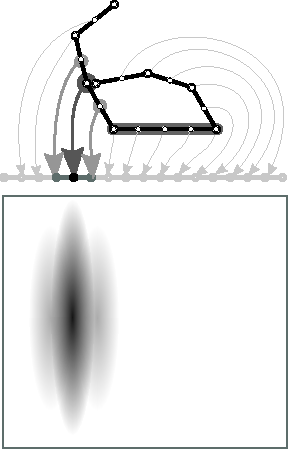
\includegraphics[scale=1.0]{sensoryinput}
\caption{}
\label{fig:sensory-input}
\end{figure}


 In the current implementatiion the GC is  a self organizing map (SOM).   

The model is based on five components: (1) a competitive neural network, supporting the acquisition of abstract representations based on experienced changes in the sensory input; (2) a selector that on the basis on competence-based intrinsic motivations (CB-IMs) determines the pursued goal and which motor resources will be trained to obtain that goal; (3) an echo-state neural network that controls the movements of the robot and supports the acquisition of the motor skills; (4) a predictor of the accomplishment of the pursued goal, used to measure the improvement of the system competence; (5) the generator of the CB-IM signal that biases the activity of the selector.
 
\subsection{Implementation details}
\label{sec:Implementation}

\subsection{Setup}
\label{sec:Setup}
 
\section{Results}
\label{sec:Results}
%Performance
 
%Stability
 
%Modulating kohonen maps
 
%predictions

\section{Predictions of the model}
\label{sec:Predictions}
\input{predictions}

\section{Discussion and future works}
\label{sec:Discussion}
\input{discussion}

\section*{Conflict of Interest Statement}
%All financial, commercial or other relationships that might be perceived by the academic community as representing a potential conflict of interest must be disclosed. If no such relationship exists, authors will be asked to confirm the following statement: 

The authors declare that the research was conducted in the absence of any commercial or financial relationships that could be construed as a potential conflict of interest.

\section*{Author Contributions}

The Author Contributions section is mandatory for all articles, including articles by sole authors. If an appropriate statement is not provided on submission, a standard one will be inserted during the production process. The Author Contributions statement must describe the contributions of individual authors referred to by their initials and, in doing so, all authors agree to be accountable for the content of the work. Please see  \href{http://home.frontiersin.org/about/author-guidelines#AuthorandContributors}{here} for full authorship criteria.

\section*{Funding}
This project has received funding from the European Union?s Horizon 2020 Research and Innovation Program under Grant Agreement no. 713010 (GOAL-Robots - Goal-based Open-ended Autonomous Learning Robots).

\section*{Acknowledgments}
The authors want to thanks ...

\bibliographystyle{frontiersinSCNS_ENG_HUMS} % for Science, Engineering and Humanities and Social Sciences articles, for Humanities and Social Sciences articles please include page numbers in the in-text citations
%\bibliographystyle{frontiersinHLTH&FPHY} % for Health, Physics and Mathematics articles
\bibliography{paper}
\end{document}
